\documentclass[a4paper]{jpconf}
\bibliographystyle{iopart-num}
\usepackage{amsmath}
\usepackage{citesort}
\usepackage{subfigure}
\usepackage{graphicx}
\graphicspath{{fig/}}
\usepackage{ifpdf}
\ifpdf\usepackage{epstopdf}\fi
\usepackage[export]{adjustbox}

%----------------------------------------------------- 
%\usepackage{soul,ulem,color,xspace,bm}
% Andrei's commands
% Suggest to remove
%\newcommand{\asrm}[1]{{\color{magenta}\sout{#1}}}
% Suggest to insert
%\newcommand{\as}[1]{\color{cyan}#1\xspace\color{black}}
% Suggest to replace
%\newcommand{\asrp}[2]{\asrm{#1} \as{#2}}
% Comment
%\newcommand{\ascm}[1]{{\color{green}\;AS: #1}}
%------------------------------------------------------

\begin{document}
\title{Particle-in-cell simulation of ion and electron acceleration in trans-relativistic shocks.}

\author{V I Romansky$^{1,2}$, A M Bykov$^1$, S M Osipov$^1$ and P E Gladilin$^1$}

\address{$^1$ Ioffe Institute, 26 Politekhnicheskaya st., St. Petersburg 194021, Russia}
\address{$^2$ 
Sternberg Astronomical Institute, Moscow State University
 Universitetsky pr., 13, Moscow 119234, Russia}

\ead{romanskyvadim@gmail.com}

\begin{abstract}
The problem of Cosmic Ray (CR) origin and acceleration is a widely discussed problem of
modern astrophysics. It is considered that most likely CR sources are 
shock waves in supernova remnants or jets. One of the methods to study particle injection and acceleration by shock
waves is a particle-in-cell computer simulation. In this paper we present results of
simulations of relativistic shock waves with low lorenz-factor, based on our self-developed implicit particle-in-cell code. 
\end{abstract}
\section{Introduction}
One of the possible sources of high-energy cosmic rays are shock waves in astrophysical collisionless plasma due to the diffusive shock acceleration (DSA) mechanism, see \cite{Bell1978}, \cite{Blandford1978}. Strong magnetic fields are necessary for effective acceleration of charged particles and the observations of the synchrotron emission from supernova remnants (SNRs) show, that the magnetic field there is about 100 times stronger then the interstellar field (see for example \cite{Berezhko2003},\cite{Uchiyama2007}). So strong fields can be produced due to instabilities in anisotropic plasma. One of the most powerful methods to explore processes in collisionless plasma is the Particle-in-Cell simulation. In this work we explore instabilities in the plasma using this method. 
We developed the implicit particle-in-cell (PIC) code, based on the scheme suggested by Lapenta et al.~\cite{Lapenta2006} and improved for the relativistic case by Noguchi et al.\cite{Noguchi2007}.
Our code is fully three dimensional and parallelized with MPI technology, which is adapted for distributed computing and can be executed on a wide class of computers.
\section{Shock wave simulation}
We studied the influence of fractions of heavy ions on the shock wave, in particular, the spectrum of particles and the shape of the shock wave. We present results of two simulations with different compositions of the plasma : pure protons and electrons in the first case and with the admixture of alpha particles in the second case. Initially the homogeneous flux is  moving from the right free boundary to the left. On the left side there is a reflecting super-conducting wall, which causes formation of shock wave. Simulations are one-dimensional and have following parameters: initial velocity $v = 0.2c$, number densities $n_e = 10^{-4} \rm{cm}^{-3}$, $n_p = 10^{-4} \rm{cm}^{-3}$ in the first simulation and $n_e = 10^{-4} \rm{cm}^{-3}$, $n_p = 0.6\cdot10^{-4} \rm{cm}^{-3}$, $n_\alpha = 0.2\cdot10^{-4} \rm{cm}^{-3}$ in the second, temperature $5\cdot10^8 \rm{K}$, magnetic field $B_\parallel = 10^{-4} \rm{G}, B_\perp= 0.7\cdot10^{-4} \rm{G}$, the full size of the box $L = 1\cdot10^{12} \rm{cm}$, the number of cells $N=2\cdot10^4$. Electron mass is reduced to $m_e = \frac{m_p}{20}$. The full time of simulation is $T = 2000 {\omega_p}^{-1}$.
\begin{figure}[h!]
	\centering
	\begin{minipage}{0.49\textwidth}
		\centering
		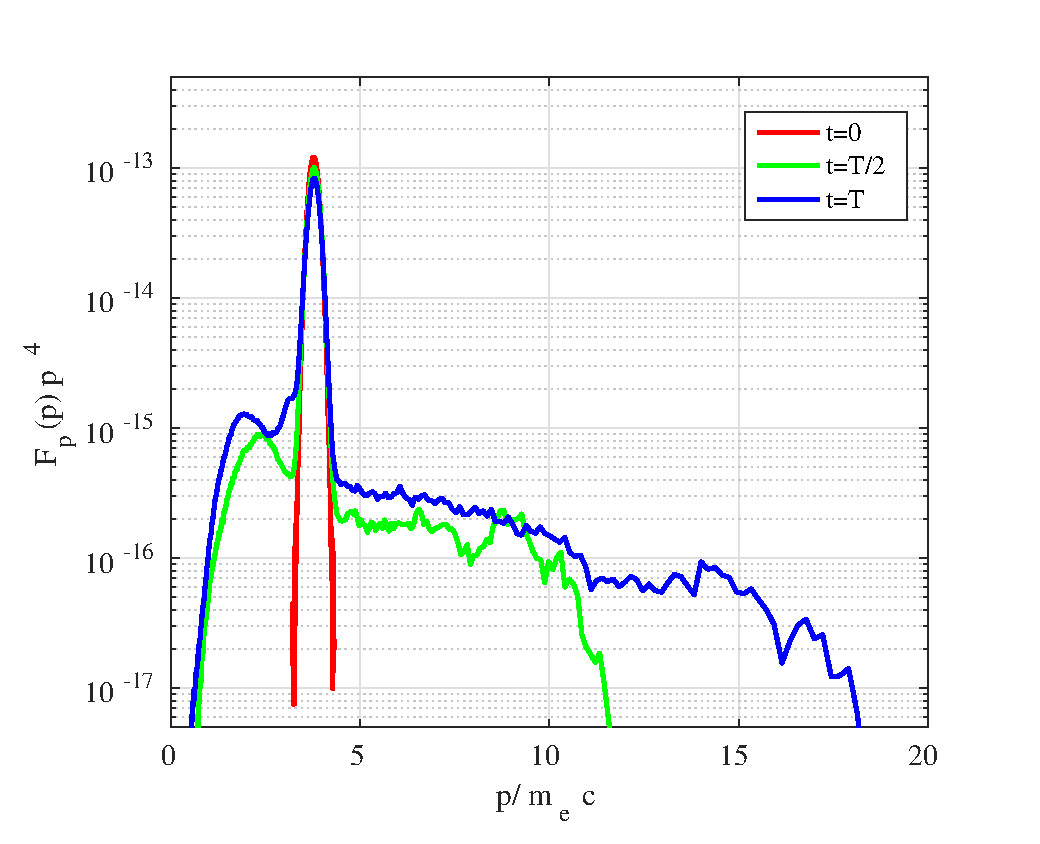
\includegraphics[width=0.98\textwidth]{fig/protons.eps} 
		\caption{Distribution of protons in the simulation without alpha particles.}
		\label{protons}
	\end{minipage}\hfill
	\begin{minipage}{0.49\textwidth}
		\centering
		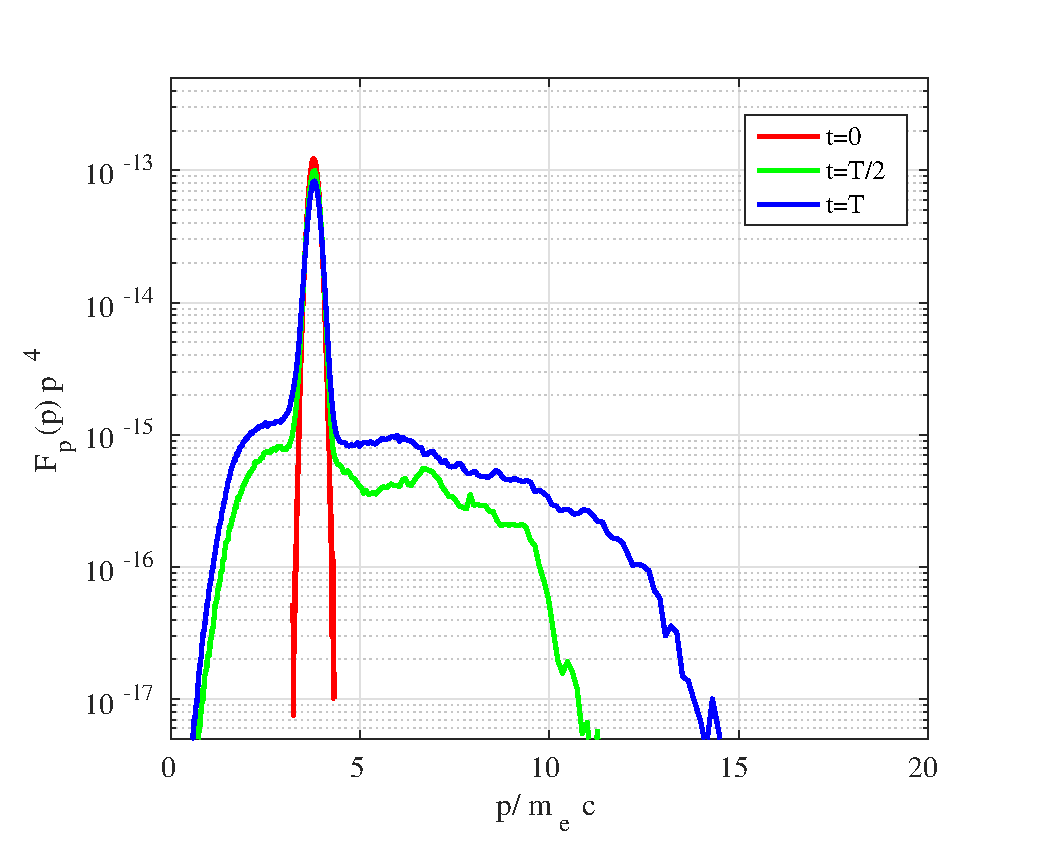
\includegraphics[width=0.98\textwidth]{fig/protons_with_He.eps} 
		\caption{Distribution of protons in the simulation with alpha particles.}
		\label{protons_with_alpha}
	\end{minipage}
\end{figure}
\begin{figure}[h!]
	\centering
	\begin{minipage}{0.49\textwidth}
		\centering
		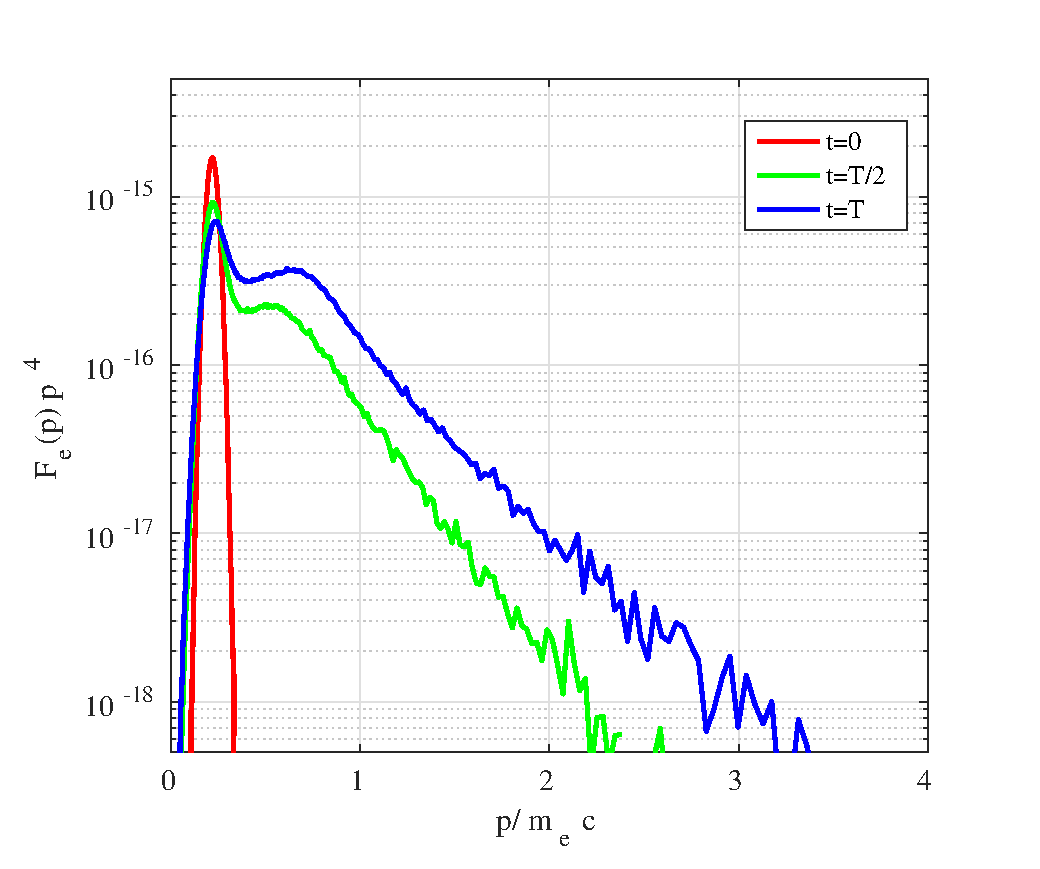
\includegraphics[width=0.98\textwidth]{fig/electrons.eps} 
		\caption{Distribution of electrons in the simulation without alpha particles.}
		\label{electrons}
	\end{minipage}\hfill
	\begin{minipage}{0.49\textwidth}
		\centering
		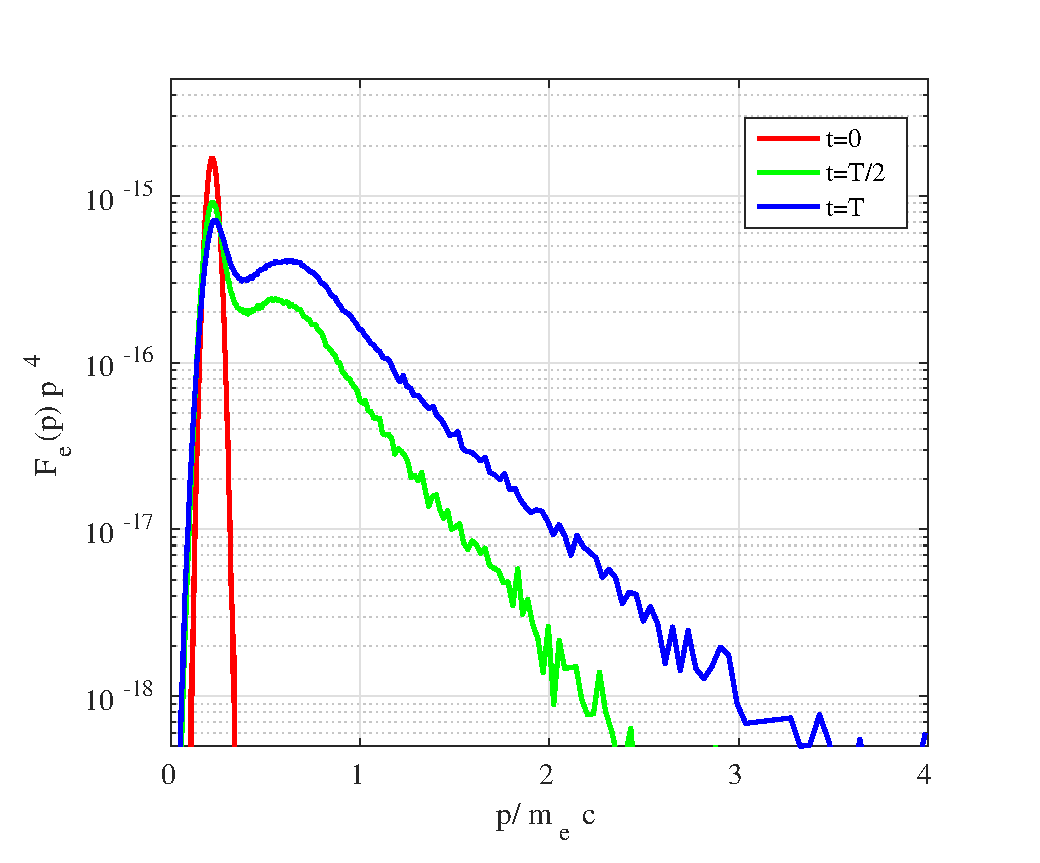
\includegraphics[width=0.98\textwidth]{fig/electrons_with_He.eps} 
		\caption{Distribution of electrons in the simulation with alpha particles.}
		\label{electrons_with_alpha}
	\end{minipage}
\end{figure}

The results presented in Figures \ref{protons}-\ref{electrons_with_alpha} show that the values of $F(p)p^4$ for high energies are much greater for protons, than for electrons in both simulations. Also electrons need much more time to be accelerated and to form spectrum $\propto p^{-4}$. It means that protons are injected into the acceleration process more efficiently, and it is consistent with the work of Park et al. {\cite{Park2015}}. Also we have shown that minority of heavy ions increases the spectrum of protons and do not have influence on the spectrum of electrons. It can be explained by the fact, that heavy ions form the large scale turbulence and protons can efficiently scatter on this turbulence. Otherwise for electrons turbulence produced by protons is already enough large-scale  and the influence of heavy ions is neglectable. 

\section{Conclusions}
In this paper we presented the developed 3D implicit particle-in-cell code, which can be applied for various problems in the collisionless plasma. We have tested it and obtained results, that are consistent with theoretical predictions. We studied the influence of admixture of heavy ions on the evolution of the shock wave and simulations have shown that the presence of heavy ions increases the number of accelerated particles. Further research is necessary in order to study this phenomena in detail.
\ack
A M Bykov, P E  Gladilin and S M  Osipov have developed the implicit fields solver module, which provides conservation of the divergenceless magnetic field. 
V I Romansky acknowledges support from RSF grant 16-12-10519 which was used to develop the
particle mover, parallelization and perform the testing of the code.


The results of the work were obtained using computational resources of Peter the Great Saint-Petersburg Polytechnic University Supercomputing Center (http://www.spbstu.ru).
\section*{References}
\begin{thebibliography}{20}
\bibitem{Bell1978} Bell A R 1978 \textit{MNRAS} \textbf{182} 147
\bibitem{Blandford1978} Blandford R D and Ostriker J P 1978 \textit{Astrophys. J.} \textbf{221} L29 
\bibitem{Berezhko2003} Berezhko E G, Ksenofontov L T and V{\"o}lk H J  2003 \textit{A}{\&}\textit{A} \textbf{412} L11
\bibitem{Uchiyama2007} Uchiyama Y, Aharonian F A, Tanaka T, Takahashi T and Maeda Y 2007 \textit{Nature} \textbf{449} 576
\bibitem{Lapenta2006} Lapenta G, Brackbill J U and Ricci P 2006 \textit{Phys. Plasmas} \textbf{13} 055904
\bibitem{Noguchi2007} Noguchi K, Tronci C, Zuccaro G and Lapenta G 2007 \textit{Phys. Plasmas} \textbf{14} 042308
\bibitem{Weibel1959} Weibel E S 1959 \textit{Phys. Rev. Lett.} \textbf{2} 83
\bibitem{Yoon1987} Yoon P H and Davidson R C 1987 \textit{Phys. Rev. A} \textbf{35} 2718
\bibitem{Park2015} Park J, Caprioli D and Spitkovsky A 2015 \textit{Phys. Rev. Lett.} \textbf{114} 085003
\end{thebibliography}
\end{document}